En esta sección se presentarán diversos artículos de investigación o tesis que abordan diversas técnicas y enfoques utilizados para afrontar problemas similares al de esta tesis. Vease el anexo 3 (insertar referencia)

\subsection{Deep Convolutional Neural Networks for Detecting COVID-19 Using Medical Images: A Survey \citep{sharma2020deep}} 

\subsubsection{Planteamiento del Problema}

En diciembre de 2019, el COVID-19, causado por el virus SARS-CoV-2, se propagó rápidamente, representando una grave amenaza para la salud pública a nivel mundial. La detección temprana y precisa es crucial para un tratamiento efectivo. Los métodos tradicionales, como las pruebas virales y de sangre, tienen limitaciones en sensibilidad y tiempo, por lo que se investiga el uso de deep learning aplicado a imágenes médicas (Rayos X, Tomografía Computarizada (CT) y Ultrasonido (US)) para mejorar la precisión y velocidad de diagnóstico.

\subsubsection{Objetivos}
\begin{itemize}
 \item Evaluar el uso de redes neuronales convolutivas (CNN) para mejorar la detección del COVID-19 a través de imágenes médicas.
 \item Comparar diferentes arquitecturas de CNN, como VGG, ResNet y DenseNet, en términos de precisión y rapidez en el diagnóstico. 
\item Analizar la efectividad de la transferencia de aprendizaje utilizando modelos preentrenados en grandes bases de datos. 
\end{itemize}

\subsubsection{Fundamento Teórico}

La implementación de deep learning en la medicina ha demostrado ser revolucionaria en el análisis de imágenes médicas, proporcionando una herramienta poderosa para la detección y diagnóstico de enfermedades. Las CNN son particularmente efectivas debido a su capacidad para reconocer patrones complejos en los datos de imagen. La transferencia de aprendizaje permite utilizar modelos preentrenados y ajustarlos para tareas específicas, mejorando significativamente la eficiencia y precisión del diagnóstico.

\subsubsection{Metodología empleada por los autores}

\paragraph{Modelos y Datasets Utilizados}

\begin{itemize}
\item Se utilizaron CNNs (VGG16, DenseNet, ResNet) aplicadas a datasets como COVIDx.
\item Los datos fueron preprocesados mediante normalización y aumento de datos para mejorar la calidad y variabilidad de las imágenes.
\end{itemize}

\begin{figure}[H]
    \centering
    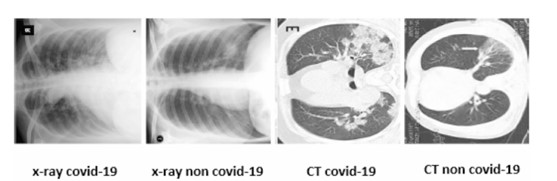
\includegraphics[width=0.9\textwidth]{images_repo/patronescovid.jpg}
    \caption{COVID-19 patterns to predict. Fuente: \cite{sharma2020deep}}
    \label{fig:COVID19_patterns}
\end{figure}

\paragraph{Evaluación de Modelos}

\begin{itemize}
\item Los modelos fueron evaluados utilizando métricas como precisión, sensibilidad, especificidad y AUC.
\item Se llevaron a cabo experimentos comparativos para determinar la arquitectura más efectiva en la detección del COVID-19.
\end{itemize}

\paragraph{Técnicas de Preprocesamiento}

\begin{itemize}
\item La normalización de imágenes fue esencial para asegurar que los datos estuvieran en un rango común, mejorando la estabilidad del entrenamiento.
\item El aumento de datos incluyó técnicas como rotación, escalado y traslación para aumentar la variabilidad y robustez del modelo.
\end{itemize}
\subsubsection{Resultados obtenidos}

\paragraph{Avances en la Detección Automatizada}

\begin{itemize}
\item Los modelos de deep learning demostraron igualar o superar la precisión de los métodos tradicionales, ofreciendo diagnósticos más rápidos y precisos.
\item  La arquitectura ResNet mostró una superioridad en términos de precisión y capacidad de generalización en comparación con VGG y DenseNet.
\end{itemize}
\paragraph{Impacto Clínico}

\begin{itemize}
\item  La implementación de estos sistemas automatizados puede mejorar la detección temprana y reducir la carga de trabajo manual, permitiendo a los profesionales de la salud centrarse en casos más complejos.
\item Los resultados sugieren una integración potencial de estos modelos en sistemas de salud reales para pruebas clínicas a gran escala.
\end{itemize}

\paragraph{Futuras Direcciones}

\begin{itemize}
\item  La investigación futura se centrará en la integración de estos modelos en sistemas de salud reales para pruebas clínicas a gran escala.
\item  Se explorará la combinación de imágenes médicas con otros datos clínicos para mejorar aún más la precisión y eficiencia del diagnóstico.
\end{itemize}

\begin{figure}[H]
    \centering
    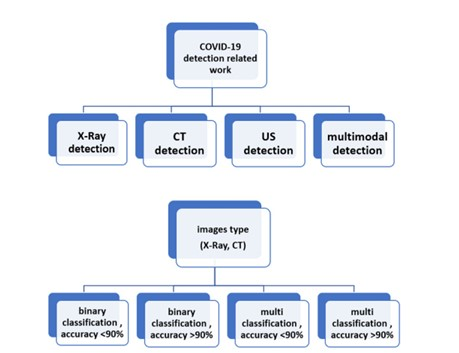
\includegraphics[width=0.9\textwidth]{images_repo/ESTRUCTURADETECCIONCOVID.jpg}
    \caption{COVID-19 detection related work. Fuente: \cite{sharma2020deep}}
    \label{fig:COVID19_diagn}
\end{figure}

\FloatBarrier

\subsection{Heart Disease Detection Using Machine Learning and Deep Learning Techniques \citep{jiang2020heart}}

\subsubsection{Planteamiento del Problema}

Las enfermedades del corazón son una de las principales causas de muerte a nivel mundial, con aproximadamente 17.9 millones de muertes registradas anualmente. Detectar la presencia de enfermedades del corazón de manera temprana es crucial para monitorear y tratar a los pacientes a tiempo y así salvar vidas. Esta investigación tiene como objetivo utilizar técnicas de aprendizaje automático y profundo para detectar enfermedades cardíacas, mejorando la precisión y la eficacia del diagnóstico.

\subsubsection{Objetivos}
\begin{itemize}
 \item Desarrollar y evaluar modelos de aprendizaje automático y profundo para la detección de enfermedades cardíacas.
 \item Comparar el rendimiento de diferentes algoritmos de machine learning y deep learning.
 \item Optimizar los modelos para su implementación práctica en entornos clínicos.
\end{itemize}

\subsubsection{Fundamento Teórico}

La implementación de técnicas de machine learning (ML) y deep learning (DL) en la medicina ha permitido avances significativos en el diagnóstico de enfermedades. Estos métodos analizan grandes volúmenes de datos médicos y son capaces de identificar patrones complejos que pueden indicar la presencia de enfermedades. Las redes neuronales convolutivas (CNN) y otros modelos de ML, como SVM y logistic regression, son particularmente efectivos en la clasificación de datos médicos.

\subsubsection{Metodología empleada por los autores}

\paragraph{Modelos Utilizados}

\begin{itemize}
\item Modelos de aprendizaje automático: SVM, logistic regression, decision tree.
\item Modelos de aprendizaje profundo: FFNN, LSTM.
\end{itemize}

\paragraph{Origen de los Datos}

\begin{itemize}
\item Los datos provinieron de un conjunto de datos con 1026 registros, que incluían diversas características médicas relevantes.
\end{itemize}

\begin{figure}[H]
    \centering
    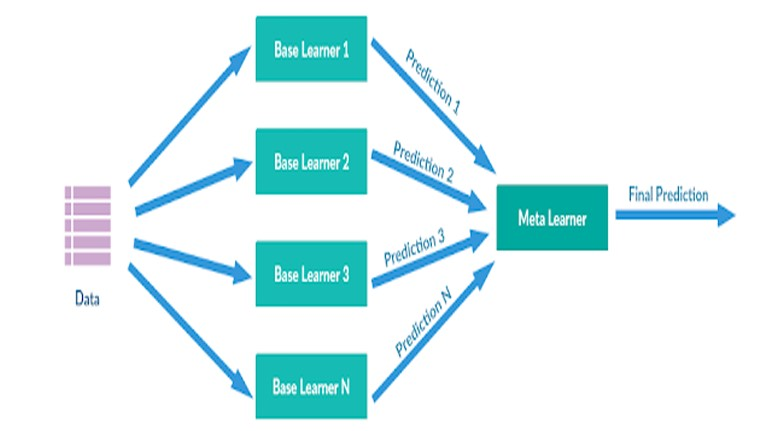
\includegraphics[width=0.9\textwidth]{images_repo/stacking.jpg}
    \caption{Tratamiento de la información propuesto. Fuente: \cite{jiang2020heart}}
    \label{Tratamiento de la información propuesto}
\end{figure}

\paragraph{Validación y Evaluación}

\begin{itemize}
\item Se aplicaron técnicas de validación cruzada para evaluar el rendimiento de los modelos.
\item Las métricas utilizadas incluyeron precisión, sensibilidad, especificidad y AUC para una evaluación exhaustiva.
\end{itemize}

\paragraph{Selección y Preprocesamiento de Características}

\begin{itemize}
\item Métodos utilizados: matriz de correlación, puntaje de Fisher.
\item Normalización de datos para asegurar que todas las características estuvieran en el mismo rango.
\end{itemize}

\paragraph{Optimización de Modelos}

\begin{itemize}
\item Ajuste fino de hiperparámetros para optimizar el rendimiento.
\item Cuantificación de parámetros para reducir el tamaño del modelo y mejorar la eficiencia del entrenamiento.
\end{itemize}

\begin{figure}[H]
    \centering
    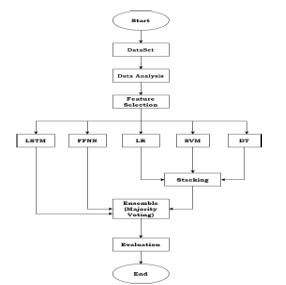
\includegraphics[width=0.7\textwidth]{images_repo/modelopropuesto.jpg}
    \caption{Modelo propuesto para el desarrollo. Fuente: \cite{jiang2020heart}}
    \label{Propossed model}
\end{figure}

\subsubsection{Resultados obtenidos}

\paragraph{Precisión de los Modelos}

\begin{itemize}
\item Los modelos de deep learning, en particular FFNN y LSTM, mostraron una alta precisión en la detección de enfermedades cardíacas.
\item Los modelos de machine learning, como SVM y logistic regression, también demostraron ser efectivos, aunque con menor precisión comparada.
\end{itemize}

\paragraph{Eficiencia y Aplicabilidad Clínica}

\begin{itemize}
\item La implementación de estos modelos en sistemas automatizados puede reducir significativamente la carga de trabajo manual en entornos clínicos.
\item Los modelos demostraron ser capaces de proporcionar diagnósticos rápidos y precisos, facilitando la toma de decisiones médicas.
\end{itemize}

\paragraph{Direcciones Futuras}

\begin{itemize}
\item Integrar estos modelos en sistemas de salud reales para pruebas clínicas a gran escala.
\item Explorar la combinación de datos médicos con otras fuentes de información para mejorar la precisión y eficiencia del diagnóstico.
\end{itemize}

\begin{figure}[H]
    \centering
    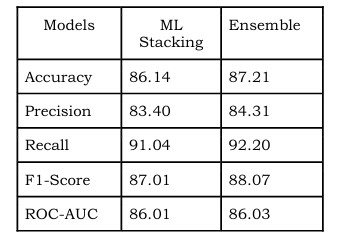
\includegraphics[width=0.9\textwidth]{images_repo/METRICASRENDIMIENTO.jpg}
    \caption{Rendimiento del modelo propuesto. Fuente: \cite{jiang2020heart}}
    \label{Rendimiento del modelo propuesto}
\end{figure}


\subsection{Monitoring and Recognition of Heart Health using Heartbeat Classification with Deep Learning and IoT \citep{arulkumar2023monitoring}}

\subsubsection{Planteamiento del Problema}

Las enfermedades cardiovasculares, como la arritmia y el infarto de miocardio, representan graves problemas de salud que pueden ser mortales si no se detectan y tratan a tiempo. La detección temprana y precisa es crucial para un tratamiento efectivo. El objetivo de este estudio es utilizar técnicas de aprendizaje profundo y el Internet de las cosas (IoT) para mejorar la detección y clasificación de latidos cardíacos, lo que permite identificar problemas de salud cardíaca de manera automática y precisa.

\subsubsection{Objetivos}
\begin{itemize}
    \item Utilizar técnicas de deep learning para mejorar la detección de arritmias y otras enfermedades cardíacas.
    \item Implementar IoT para la recolección de datos en tiempo real y monitoreo continuo de la salud cardíaca.
    \item Evaluar la precisión y efectividad del sistema propuesto utilizando el dataset MIT-BIH arrhythmia.
\end{itemize}

\subsubsection{Fundamento Teórico}

El avance en las técnicas de aprendizaje profundo y la inteligencia artificial ha permitido mejorar significativamente el diagnóstico médico, especialmente en la clasificación de señales de electrocardiograma (ECG). El uso de redes neuronales convolutivas (CNN) y otras arquitecturas de deep learning permite la detección precisa de patrones en las señales cardíacas, facilitando la identificación de arritmias y otras anomalías.

\subsubsection{Metodología empleada por los autores}

\paragraph{Adquisición y Procesamiento de Datos}

\begin{itemize}
    \item \textbf{Sensores Médicos:} Los parámetros biomédicos se calculan utilizando sensores para proporcionar mediciones precisas de los parámetros físicos. Estos datos se obtienen mediante dispositivos portátiles para monitorear la salud del corazón y detectar anomalías en su funcionamiento.
    \item \textbf{Procesamiento de Datos:} Incluye la recolección de datos de señales ECG a través de conductores y electrodos. El ruido se elimina mediante la Transformada Wavelet Discreta (DWT), lo que mejora la calidad del conjunto de datos.
\end{itemize}

\paragraph{Clasificación y Análisis de Datos}

\begin{itemize}
    \item \textbf{Redes Neuronales Convolutivas (CNN):} Utilización de modelos CNN 1D para aplicaciones en tiempo real, compuestos por varias capas utilizadas para el procesamiento y extracción de características.
    \item \textbf{Memoria Bidireccional a Largo Plazo (Bi-LSTM):} Modelo que incluye direcciones hacia adelante y hacia atrás para la acumulación y procesamiento de datos, mejorando la precisión del etiquetado de secuencias.
\end{itemize}

\begin{figure}[H]
    \centering
    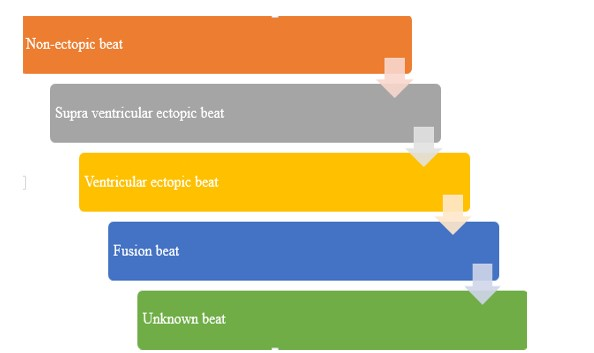
\includegraphics[width=0.9\textwidth]{images_repo/clasilatid.jpg}
    \caption{Clasificación de los latidos. Fuente: \cite{arulkumar2023monitoring}}
    \label{Clasificación de los latidos}
\end{figure}

\paragraph{Evaluación del Sistema}

\begin{itemize}
    \item \textbf{Evaluación del Desempeño:} Uso de métricas como precisión, sensibilidad, especificidad y AUC para evaluar la efectividad del sistema.
    \item \textbf{Validación y Pruebas:} El sistema se entrenó y validó utilizando el dataset MIT-BIH arrhythmia, obteniendo altos niveles de precisión y eficiencia.
\end{itemize}

\begin{figure}[H]
    \centering
    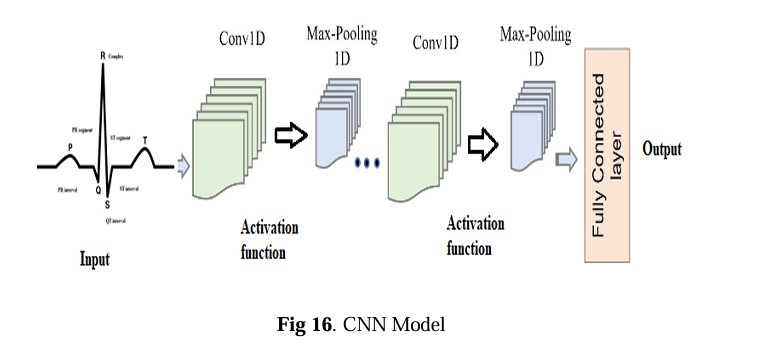
\includegraphics[width=0.9\textwidth]{images_repo/CNN.jpg}
    \caption{Modelo de CNN. Fuente: \cite{arulkumar2023monitoring}}
    \label{Modelo de CNN}
\end{figure}

\subsubsection{Resultados obtenidos}

\begin{itemize}
    \item \textbf{Avances en la Detección Automatizada:} Los modelos de deep learning demostraron ser altamente precisos en la detección de arritmias y otras enfermedades cardíacas, con una precisión del 99.98%.
    \item \textbf{Impacto en la Salud Clínica:} La implementación de estos sistemas automatizados mejora la detección temprana y reduce la carga de trabajo manual, permitiendo a los profesionales de la salud centrarse en casos más complejos.
    \item \textbf{Futuras Direcciones:} La investigación futura se centrará en la integración de estos modelos en sistemas de salud reales para pruebas clínicas a gran escala y la exploración de nuevas técnicas de procesamiento de señales y aprendizaje profundo.
\end{itemize}

\begin{figure}[H]
    \centering
    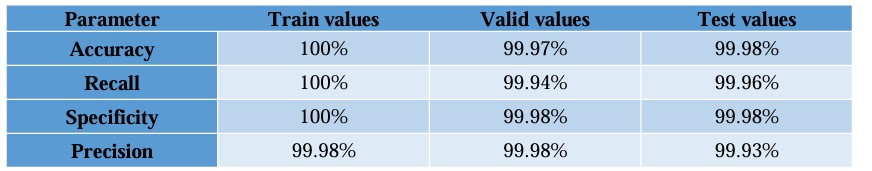
\includegraphics[width=0.9\textwidth]{images_repo/PERFORMAC.jpg}
    \caption{Tabla de rendimiento del modelo. Fuente: \cite{arulkumar2023monitoring}}
    \label{Tabla de rendimiento del modelo}
\end{figure}


\subsection{Advances in Deep Learning: From Diagnosis to Treatment \citep{huang2023advances}}

\subsubsection{Planteamiento del Problema}

El aprendizaje profundo ha revolucionado el campo del diagnóstico y tratamiento médico, alcanzando niveles de precisión comparables a los de los profesionales médicos en diversas tareas diagnósticas. Este estudio investiga el uso de modelos de aprendizaje profundo para integrar diferentes formas de datos médicos y proporcionar sugerencias diagnósticas y de tratamiento precisas y en tiempo real.

\subsubsection{Objetivos}

\begin{itemize}
    \item Explorar la integración de modelos de aprendizaje profundo en sistemas de diagnóstico y tratamiento médico.
    \item Evaluar la efectividad de los modelos de aprendizaje profundo en la mejora de la precisión diagnóstica y la eficiencia del tratamiento.
    \item Analizar la colaboración entre médicos y máquinas en el contexto de la atención médica personalizada.
\end{itemize}

\subsubsection{Fundamento Teórico}

El uso de deep learning en la medicina ha crecido exponencialmente en los últimos años, logrando una precisión similar a la de los médicos en diversas tareas diagnósticas. Los modelos de deep learning pueden integrar diferentes formas de datos médicos, como imágenes, registros electrónicos de salud, genómica y texto médico, para proporcionar salidas útiles basadas en la información del paciente. Estos modelos tienen el potencial de transformar los sistemas de diagnóstico y tratamiento al proporcionar capacidades de razonamiento en tiempo real en escenarios quirúrgicos complejos.


\subsubsection{Metodología empleada por los autores}

\paragraph{Modelos y Datasets Utilizados}

\begin{itemize}
    \item Evaluación de modelos avanzados de deep learning como R-CNN, U-Net y GPT-4 aplicados a conjuntos de datos médicos variados.
    \item Integración de diversas formas de datos médicos, incluyendo imágenes médicas, registros electrónicos de salud, y datos genómicos.
\end{itemize}

\paragraph{Desarrollo de Modelos de Fundamento Médico}

\begin{itemize}
    \item Utilización de grandes conjuntos de datos de entrenamiento para mejorar la capacidad de razonamiento de los modelos.
    \item Implementación de modelos que integran múltiples formas de información médica para proporcionar diagnósticos y sugerencias de tratamiento precisas.
\end{itemize}

\paragraph{Automatización en Procedimientos Quirúrgicos}

\begin{itemize}
    \item Uso de aprendizaje por refuerzo para permitir la operación autónoma de robots durante procedimientos quirúrgicos simples.
    \item Desarrollo de dispositivos quirúrgicos integrados con tecnología de modelo de fundamento médico para mejorar la toma de decisiones diagnósticas y terapéuticas.
\end{itemize}

\subsubsection{Resultados obtenidos}

\paragraph{Avances en Diagnóstico y Tratamiento Automatizado}

\begin{itemize}
    \item Los modelos de deep learning han demostrado igualar o superar la precisión de los métodos tradicionales en tareas diagnósticas, ofreciendo diagnósticos y sugerencias de tratamiento más rápidos y precisos.
    \item Los modelos de fundamento médico muestran un gran potencial para realizar tareas más diversas y desafiantes al integrar múltiples formas de datos médicos.
\end{itemize}

\paragraph{Colaboración entre Médicos y Máquinas}

\begin{itemize}
    \item La implementación de sistemas automatizados puede mejorar la eficiencia y precisión del diagnóstico, reduciendo la carga de trabajo manual de los profesionales de la salud.
    \item Los médicos deben comprender los principios y riesgos técnicos de los métodos de deep learning y dominar los procedimientos para integrarlos en la práctica clínica.
\end{itemize}

\paragraph{Futuras Direcciones}

\begin{itemize}
    \item La investigación futura se centrará en la integración de modelos de fundamento médico en sistemas de salud reales para pruebas clínicas a gran escala.
    \item Desarrollo de sistemas autónomos de diagnóstico y tratamiento que puedan operar con mínima intervención humana, mejorando la precisión y personalización de la atención médica.
\end{itemize}

\subsection{A Study on Scope of Artificial Intelligence in Diagnostic Medicine \citep{santhoshkumar2023}} 

\subsubsection{Planteamiento del Problema}

El uso de técnicas de inteligencia artificial (IA) está mejorando significativamente la atención al paciente y los sistemas de salud. La capacidad de la IA para analizar grandes cantidades de datos médicos y reconocer patrones ha mostrado un potencial considerable en el diagnóstico de enfermedades. Este estudio analiza cómo las técnicas de IA, incluyendo el aprendizaje automático y profundo, pueden integrarse en la medicina diagnóstica para mejorar la precisión del diagnóstico y optimizar la atención al paciente.

\subsubsection{Objetivos}
\begin{itemize}
    \item Evaluar el impacto de la IA en el diagnóstico médico y su capacidad para mejorar la precisión y eficiencia en la detección de enfermedades.
    \item Analizar las aplicaciones actuales de la IA en la medicina diagnóstica, incluyendo el reconocimiento de imágenes, procesamiento del lenguaje natural (NLP) y análisis de datos genómicos.
    \item Examinar los desafíos éticos y técnicos asociados con la implementación de la IA en la atención médica.
\end{itemize}

\subsubsection{Fundamento Teórico}

La adopción de tecnologías avanzadas como la inteligencia artificial (IA) está provocando un cambio rápido en el sector sanitario. La IA se utiliza para crear nuevos sistemas clínicos, mejorar los datos y registros de los pacientes, e identificar diversas enfermedades. La integración de la IA con otras tecnologías digitales tiene el potencial de transformar por completo el sector sanitario, mejorando los resultados de los pacientes, reduciendo los costos y permitiendo una atención más individualizada y eficaz.
\begin{figure}[H]
    \centering
    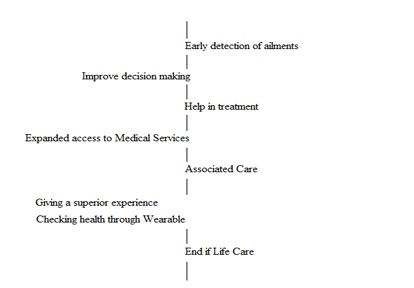
\includegraphics[width=0.9\textwidth]{images_repo/USOSIA.jpg}
    \caption{Clasificaciones de los diferentes uso a la IA en la medicina. Fuente: \cite{santhoshkumar2023}}
    \label{Clasificaciones de los diferentes uso a la IA en la medicina}
\end{figure}


\subsubsection{Metodología empleada por los autores}

\paragraph{Reconocimiento de Imágenes}
\begin{itemize}
    \item Uso de algoritmos de IA para analizar imágenes médicas como radiografías, tomografías computarizadas (CT) y resonancias magnéticas (MRI).
    \item Identificación de anomalías que podrían ser indicativas de enfermedades, como el cáncer de piel y el cáncer de pulmón.
\end{itemize}

\paragraph{Procesamiento del Lenguaje Natural (NLP)}
\begin{itemize}
    \item Análisis de registros de salud electrónicos (EHR) y patrones de lenguaje para identificar indicios de enfermedades.
    \item Detección temprana de sepsis y signos iniciales de la enfermedad de Alzheimer en patrones de habla.
\end{itemize}

\paragraph{Análisis de Datos Genómicos}
\begin{itemize}
    \item Uso de IA para analizar datos genéticos y encontrar mutaciones o variaciones que podrían indicar riesgos de enfermedades.
    \item Identificación de marcadores genéticos para el cáncer de mama y diagnóstico de trastornos genéticos raros.
\end{itemize}

\begin{figure}[H]
    \centering
    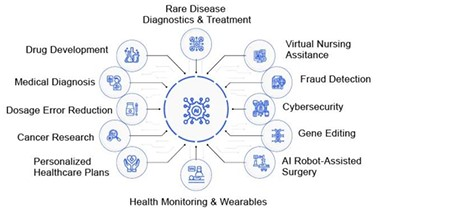
\includegraphics[width=0.9\textwidth]{images_repo/APLICACION.jpg}
    \caption{Aplicación de la IA en la rama de la SALUD. Fuente: \cite{santhoshkumar2023}}
    \label{Aplicación de la IA en la rama de la SALUD}
\end{figure}

\subsubsection{Resultados obtenidos}

\paragraph{Avances en la Detección Automatizada}
\begin{itemize}
    \item La IA ha mostrado un potencial considerable para mejorar la precisión y rapidez del diagnóstico de enfermedades.
    \item Los sistemas de IA pueden ayudar a reducir falsos positivos y falsos negativos, mejorando los resultados de los pacientes.
\end{itemize}

\paragraph{Impacto Clínico}
\begin{itemize}
    \item La implementación de IA puede mejorar la toma de decisiones clínicas y reducir la carga de trabajo manual de los profesionales de la salud.
    \item La IA tiene el potencial de transformar la atención médica al permitir diagnósticos más precisos y tratamientos personalizados.
\end{itemize}

\paragraph{Desafíos y Futuras Direcciones}
\begin{itemize}
    \item Asegurar la privacidad y seguridad de los datos del paciente sigue siendo un desafío importante.
    \item La investigación futura se centrará en el desarrollo de prácticas éticas y responsables para la implementación de la IA en la atención médica.
\end{itemize}
